 % The main file for CAMP reports
 % Don't put any content in here.
 % Don't even include content files by using \input or \inlcude.
 % Put your content to TEXT.TEX or include it there using \input.
 % Uses:
 %		SETTINGS.TEX	contains the settings for this document
 %		COMMANDS.TEX	contains commands which can be used while writing
 %		INFO.TEX			contains the author, title and so on for the cover
 %		COVER.TEX			formats the front cover of the document
 %		ABSTRACT.TEX	contains the abstract to be included (if needed)
 %		TEXT.TEX			contains the actual content of the document
 %		BIB.BIB				containt the BibTeX entries for the document


%% Draft document mode
%% Final document
\documentclass[11pt,a4paper,bibtotoc,idxtotoc,headsepline,footsepline,footexclude,BCOR14mm,DIV13]{scrbook}

%\documentclass[11pt,a4paper,bibtotoc,idxtotoc,headsepline,footsepline,footexclude,BCOR20mm,DIV10]{scrbook}

% KOMA-Optionen:
%  bibtotoc: include bibliography in table of contents
%  idxtotoc: include index in table of contents
%  headsepline: use horizontalline under heading
%  BCOR: binding correcion (Bindungskorrektur) (e.g.: BCOR5mm)
%  DIV: Number of sheet sections (used for layout) (e.g.: DIV12)



% include title and author information for the cover
% Set here the title, authors and other stuff to be used for the cover
% This file is used by MAIN.TEX

% set title, authors and stuff for the cover
\def\doctype{Bachelor's Thesis in Informatics}
\def\title{Training a Spiking Neural Network using R-STDP to perform Autonomous Target Tracking on a Snake Car Robot}
\def\titleGer{Training von Spiking Neural Networks f\"ur die Automatische Zielverfolgung auf einem Schlangen Roboter mit R-STDP}
\def\author{Ren\'e Romen}
\def\date{\today}

% text to appear in the footer
\def\footertext{}


% include settings
% Included by MAIN.TEX
% Defines the settings for the CAMP report document

\renewcommand{\sectfont}{\normalfont \bfseries}        % Schriftart der Kopfzeile

% manipulate footer
\usepackage{scrpage2}
\pagestyle{scrheadings}
\ifoot[\footertext]{\footertext} % \footertext set in INFO.TEX
%\setkomafont{pagehead}{\normalfont\rmfamily}
\setkomafont{pagenumber}{\normalfont\rmfamily}

%% allow sophisticated control structures
\usepackage{ifthen}

% use Palatino as default font
\usepackage{palatino}

% enable special PostScript fonts
\usepackage{pifont}

% make thumbnails
\usepackage{thumbpdf}

%to use the subfigures
\usepackage{subfigure}


\usepackage{colortbl}


%% show program code\ldots
%\usepackage{verbatim}
%\usepackage{program}

%% enable TUM symbols on title page
\usepackage{styles/tumlogo}


\usepackage{multirow}

%% use colors
\usepackage{color}

%% make fancy math
\usepackage{amsmath}
\usepackage{amsfonts}
\usepackage{amssymb}
\usepackage{textcomp}
\usepackage{yhmath} % f�r die adots 
%% mark text as preliminary
%\usepackage[draft,german,scrtime]{prelim2e}

%% create an index
\usepackage{makeidx}

% for the program environment
\usepackage{float}

%% load german babel package for german abstract
%\usepackage[german,american]{babel}
\usepackage[german,english]{babel}
\selectlanguage{english}

% use german characters as well
\usepackage[utf8]{inputenc}       % allow Latin1 characters

% use initals dropped caps - doesn't work with PDF
\usepackage{dropping}

\usepackage{styles/shortoverview}
%----------------------------------------------------
%      Graphics and Hyperlinks
%----------------------------------------------------

%% check for pdfTeX
\ifx\pdftexversion\undefined
 %% use PostScript graphics
 \usepackage[dvips]{graphicx}
 \DeclareGraphicsExtensions{.eps,.epsi}
 \graphicspath{{figures/}{figures/review}} 
 %% allow rotations
 \usepackage{rotating}
 %% mark pages as draft copies
 %\usepackage[english,all,light]{draftcopy}
 %% use hypertex version of hyperref
 \usepackage[hypertex,hyperindex=false,colorlinks=false]{hyperref}
\else %% reduce output size \pdfcompresslevel=9
 %% declare pdfinfo
 %\pdfinfo { 
 %  /Title (my title) 
 %  /Creator (pdfLaTeX) 
 %  /Author (my name) 
 %  /Subject (my subject	) 
 %  /Keywords (my keywords)
 %}
 %% use pdf or jpg graphics
 \usepackage[pdftex]{graphicx}
 \DeclareGraphicsExtensions{.jpg,.JPG,.png,.pdf,.eps}
 \graphicspath{{figures/}} 
 
 %% Load float package, for enabling floating extensions
 \usepackage{float}
 
 %% allow rotations
 \usepackage{rotating}
 %% use pdftex version of hyperref
 \usepackage[pdftex,colorlinks=true,linkcolor=red,citecolor=red,%
 anchorcolor=red,urlcolor=red,bookmarks=true,%
 bookmarksopen=true,bookmarksopenlevel=0,plainpages=false%
 bookmarksnumbered=true,hyperindex=false,pdfstartview=%
 ]{hyperref}
%
%\usepackage[pdftex,colorlinks=false,linkcolor=red,citecolor=red,%
% anchorcolor=red,urlcolor=red,bookmarks=true,%
% bookmarksopen=true,bookmarksopenlevel=0,plainpages=false%
% bookmarksnumbered=true,hyperindex=false,pdfstartview=%
% ]{hyperref}
\fi




%% Fancy chapters
%\usepackage[Lenny]{fncychap}
%\usepackage[Glenn]{fncychap}
%\usepackage[Bjarne]{fncychap}

%\usepackage[avantgarde]{quotchap}

% set the bibliography style
%\bibliographystyle{styles/bauermaNum}
%\bibliographystyle{alpha}
\bibliographystyle{plain}


\DeclareMathOperator*{\argmin}{arg\,min}
\DeclareMathOperator*{\argmax}{arg\,max}



\usepackage{parskip}
%\setlength{\parskip}{3mm plus 4mm minus 4mm}
%\setlength{\parskip}{2mm plus0mm minus1mm}
%\setlength{\parindent}{0pt}
\clubpenalty = 10000
\widowpenalty = 10000



\usepackage{titlesec}
\titlespacing*{\section} {0pt}{2.5ex plus 1ex minus .2ex}{2.3ex plus .2ex}
\titlespacing*{\subsection} {0pt}{3.25ex plus 1ex minus .2ex}{1.5ex plus .2ex}
\titlespacing*{\subsubsection}{0pt}{3.25ex plus 1ex minus .2ex}{1.5ex plus .2ex}
\titlespacing*{\paragraph} {0pt}{3.25ex plus 1ex minus .2ex}{1em}
\titlespacing*{\subparagraph} {\parindent}{3.25ex plus 1ex minus .2ex}{1em}


\usepackage{listings}

\lstset{
%language=C,
basicstyle=\small\ttfamily,
%numbers=left,
%numberstyle=\tiny,
%frame=tb,
columns=fullflexible,
showstringspaces=false
}


\usepackage{color}
\usepackage{xcolor}
\usepackage{caption}
\DeclareCaptionFont{white}{\color{white}}
\DeclareCaptionFormat{listing}{\colorbox{gray}{\parbox{\textwidth}{#1#2#3}}}
\captionsetup[lstlisting]{format=listing,labelfont=white,textfont=white}



% include commands
% Commands to be used within the TUM report document
% Included by MAIN.TEX
% Please include your own cool commands here. 
% Be only sure to comment it sufficiently so others can use it.

%-------------------------------------------------------------
%                      Own Commands
%-------------------------------------------------------------


%-------------------------------------------------------------
% math stuff -------------------------------------------------

% nice R, N, C
\newcommand{\nat}{\mathbb{N}}
\newcommand{\real}{\mathbb{R}}
\newcommand{\compl}{\mathbb{C}}



% norm
\newcommand{\norm}[1]{\left\| #1 \right\|}

% un demi
\newcommand{\half}{\frac{1}{2}}

% parantheses
\newcommand{\parenth}[1]{ \left( #1 \right) }
\newcommand{\bracket}[1]{ \left[ #1 \right] }
\newcommand{\accolade}[1]{ \left\{ #1 \right\} }
%\newcommand{\angle}[1]{ \left\langle  #1 \right\rangle }

% partial derivative: %#1 function, #2 which variable
% simple / single line version
\newcommand{\pardevS}[2]{ \delta_{#1} f(#2) }
% fraction version
\newcommand{\pardevF}[2]{ \frac{\partial #1}{\partial #2} }

% render vectors: 3 and 4 dimensional
\newcommand{\veciii}[3]{\left[ \begin{array}[h]{c} #1 \\ #2 \\ #3	\end{array} \right]}
\newcommand{\veciv}[4]{\left[ \begin{array}[h]{c} #1 \\ #2 \\ #3 \\ #4	\end{array} \right]}

% render matrices: 3  dimensional (arguments in row first order)
\newcommand{\matiii}[9]{\left[ \begin{array}[h]{ccc} #1 & #2 & #3 \\ #4 & #5 & #6 \\ #7 & #8 & #9	\end{array} \right]}
%DOESN'T WORK,DON'T KNOW WHY \newcommand{\mativ}[16]{\left[ \begin{array}[h]{cccc} #1 & #2 & #3 & #4 \\ #5 & #6 & #7 & #8 \\ #9 & #10 & #11 & #12 \\ #13 & #14 & #15 & #16 \end{array} \right]}


%-------------------------------------------------------------
%-------------------------------------------------------------


%-------------------------------------------------------------
% some abreviations ------------------------------------------
\newcommand{\Reg}{$^{\textregistered}$}
\newcommand{\reg}{$^{\textregistered}$ }
\newcommand{\Tm}{\texttrademark}
\newcommand{\tm}{\texttrademark~}
\newcommand {\bsl} {$\backslash$}

%-------------------------------------------------------------
%-------------------------------------------------------------


%-------------------------------------------------------------
% formating --------------------------------------------------

% Theorem & Co environments and counters
\newtheorem{theorem}{Theorem}[chapter]
\newtheorem{lemma}[theorem]{Lemma}
\newtheorem{corollary}[theorem]{Corollary}
\newtheorem{remark}[theorem]{Remark}
\newtheorem{definition}[theorem]{Definition}
\newtheorem{equat}[theorem]{Equation}
\newtheorem{example}[theorem]{Example}
\newtheorem{algorithm}[theorem]{Algorithm}

% inserting figures
\newcommand{\insertfigure}[4]{ % Filename, Caption, Label, Width percent of textwidth
	\begin{figure}[htbp]
		\begin{center}
			\includegraphics[width=#4\textwidth]{#1}
		\end{center}
		\vspace{-0.4cm}
		\caption{#2}
		\label{#3}
	\end{figure}
}




% referecing figures

\newcommand{\refFigure}[1]{ %label
	figure \ref{#1}
}
\newcommand{\refChapter}[1]{ %label
	chapter \ref{#1}
}

\newcommand{\refSection}[1]{ %label
	section \ref{#1}
}

\newcommand{\refParagraph}[1]{ %label
	paragraph \ref{#1}
}

\newcommand{\refEquation}[1]{ %label
	equation \ref{#1}
}

\newcommand{\refTable}[1]{ %label
	table \ref{#1}
}




\newcommand{\rigidTransform}[2]
{
	${}^{#2}\!\mathbf{H}_{#1}$
}

%code, in typewriter
\newcommand{\code}[1]
 {\texttt{#1}}

% comment that appears on the border - very practical !!!
\newcommand{\comment}[1]{\marginpar{\raggedright \noindent \footnotesize {\sl #1} }}

% page clearing
\newcommand{\clearemptydoublepage}{%
  \ifthenelse{\boolean{@twoside}}{\newpage{\pagestyle{empty}\cleardoublepage}}%
  {\clearpage}}


%-------------------------------------------------------------
%-------------------------------------------------------------


\newcommand{\etAl}{\emph{et al.}\mbox{ }}

\pdfinfo{
   /Author (Ren\'e Romen)
   /Title (Training a Spiking Neural Network using R-STDP to perform Autonomous Target Tracking on a Snake Car Robot)
   /Keywords (SNN, Snake, Robot, Autonomous Target Tracking)
}

\hypersetup{%
pdftitle={Training a Spiking Neural Network using R-STDP to perform Autonomous Target Tracking on a Snake Car Robot},%
pdfauthor={Ren\'e Romen},%
pdfkeywords={SNN, Snake, Robot, Autonomous Target Tracking},%
}%

\hypersetup{
    colorlinks=false,
    pdfborder={0 0 0},
}


%\makeindex
	%% inter line spacing
%\linespread{1.0}

\makeglossary

\begin{document}

	\frontmatter
	
	
	% The front cover for the TUM report document.
% Included by MAIN.TEX


%--------------------------------------------------
% The Front Cover
%--------------------------------------------------

% The front cover for the TUM document.
% Included by MAIN.TEX


%--------------------------------------------------
% The Front Cover
%--------------------------------------------------

% correct BCOR - undo at the end !!!
\def\bcorcor{0.15cm}
\addtolength{\hoffset}{\bcorcor}

\thispagestyle{empty}

 \vspace{4cm}
\begin{center}
	       \oTUM{4cm}
	   
	   \vspace{5mm}     
%	   \huge FAKULT{\"A}T F{\"U}R INFORMATIK\\ 
	   \huge DEPARTMENT OF INFORMATICS \\
	   \vspace{0.5cm}
%	 \large DER TECHNISCHEN UNIVERSIT{\"A}T M{\"U}NCHEN\\
	\large TECHNISCHE UNIVERSIT{\"A}T M{\"U}NCHEN\\
    \vspace{1mm}
        
	\end{center}
		

\vspace{15mm}
\begin{center}

   {\Large \doctype}

  \vspace{20mm}
  
  {\huge\bf \title}\\%[3ex]
  
  
  \vspace{15mm}
  
  
  {\LARGE  \author}
  
  \vspace{10mm}
  
  \begin{figure}[h!]
  \centering
   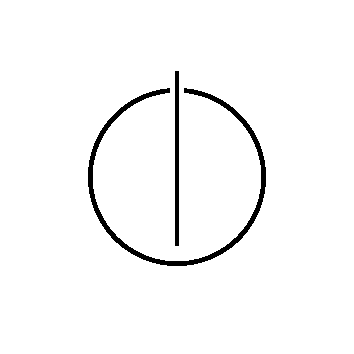
\includegraphics[width=4cm]{styles/informat.png}
  \end{figure}
  
  \end{center}

%	\clearemptydoublepage
%	
%	% The titlepage for the CAMP report document.
% Included by MAIN.TEX


%--------------------------------------------------
% The title page
%--------------------------------------------------

% correct BCOR - undo at the end !!!
\def\bcorcor{0.15cm}
\addtolength{\hoffset}{\bcorcor}

\thispagestyle{empty}

 \vspace{10mm}
\begin{center}
	       \oTUM{4cm}
	   
	   \vspace{5mm}     
	   %\huge FAKULT{\"A}T F{\"U}R INFORMATIK\\ 
	   \huge DEPARTMENT OF INFORMATICS \\
	   \vspace{0.5cm}
	 %\large DER TECHNISCHEN UNIVERSIT{\"A}T M{\"U}NCHEN\\
	 \large TECHNISCHE UNIVERSIT{\"A}T M{\"U}NCHEN\\
        
	\end{center}
		

\vspace{10mm}
\begin{center}

   {\Large \doctype}

  \vspace{10mm}
  
  {\LARGE \title}\\
  
  
  \vspace{10mm}
  
  
  {\LARGE  \titleGer}\\
  
  
  \vspace{10mm}

    %\hfill
    \begin{tabular}{ll}
	   \Large Author:     & \Large \author \\[2mm]
	   \Large Supervisor:    & \Large Prof. Dr.-Ing. habil. Alois Knoll \\[2mm]
	   \Large Advisors:	& \Large Zhenshan Bing, M.Sc.\\[2mm]
	   \Large Date:       & \Large \today
	 \end{tabular}
	 
	 \vspace{5mm}
	 
	 \begin{figure}[h!]
  \centering
   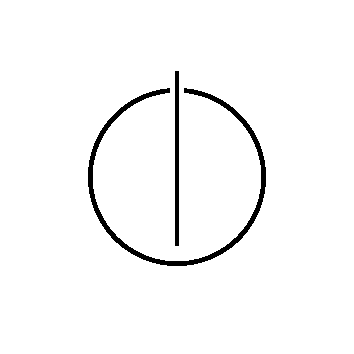
\includegraphics[width=4cm]{styles/informat.png}
  \end{figure}
   

\end{center}

% undo BCOR correction
\addtolength{\hoffset}{\bcorcor}

	
	
%	\input{components/cover_maschmeyer}
	\clearemptydoublepage
	
	% The titlepage for the CAMP report document.
% Included by MAIN.TEX


%--------------------------------------------------
% The title page
%--------------------------------------------------

% correct BCOR - undo at the end !!!
\def\bcorcor{0.15cm}
\addtolength{\hoffset}{\bcorcor}

\thispagestyle{empty}

 \vspace{10mm}
\begin{center}
	       \oTUM{4cm}
	   
	   \vspace{5mm}     
	   %\huge FAKULT{\"A}T F{\"U}R INFORMATIK\\ 
	   \huge DEPARTMENT OF INFORMATICS \\
	   \vspace{0.5cm}
	 %\large DER TECHNISCHEN UNIVERSIT{\"A}T M{\"U}NCHEN\\
	 \large TECHNISCHE UNIVERSIT{\"A}T M{\"U}NCHEN\\
        
	\end{center}
		

\vspace{10mm}
\begin{center}

   {\Large \doctype}

  \vspace{10mm}
  
  {\LARGE \title}\\
  
  
  \vspace{10mm}
  
  
  {\LARGE  \titleGer}\\
  
  
  \vspace{10mm}

    %\hfill
    \begin{tabular}{ll}
	   \Large Author:     & \Large \author \\[2mm]
	   \Large Supervisor:    & \Large Prof. Dr.-Ing. habil. Alois Knoll \\[2mm]
	   \Large Advisors:	& \Large Zhenshan Bing, M.Sc.\\[2mm]
	   \Large Date:       & \Large \today
	 \end{tabular}
	 
	 \vspace{5mm}
	 
	 \begin{figure}[h!]
  \centering
   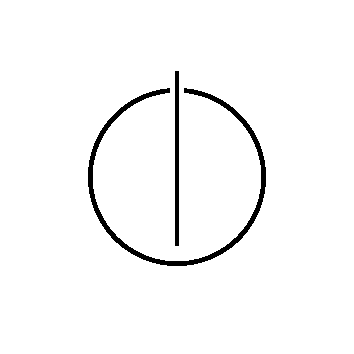
\includegraphics[width=4cm]{styles/informat.png}
  \end{figure}
   

\end{center}

% undo BCOR correction
\addtolength{\hoffset}{\bcorcor}

	
	
	\clearemptydoublepage


\thispagestyle{empty}
\selectlanguage{german}
	\vspace*{0.8\textheight}
	\noindent
	%Ich versichere, dass ich diese Diplomarbeit selbst{\"a}ndig verfasst und nur 
	%die angegebenen \\Quellen und Hilfsmittel verwendet habe.
	
	I confirm that this master's thesis is my own work and I have documented all sources and material used.
	
	\vspace{15mm}
	\noindent
	M{\"u}nchen, \today \hspace{5cm} \author
\selectlanguage{english}
\newpage

	
	%\clearemptydoublepage
\phantomsection
\addcontentsline{toc}{chapter}{Acknowledgements}	


%\chapter*{Acknowledgements}

\vspace*{2cm}

\begin{center}
{\Large \bf Acknowledgments}
\end{center}

\vspace{1cm}




If someone contributed to the thesis... might be good to thank them here.
	
	% Abstract for the TUM report document
% Included by MAIN.TEX


\clearemptydoublepage
\phantomsection
\addcontentsline{toc}{chapter}{Abstract}





\vspace*{2cm}
\begin{center}
{\Large \bf Abstract}
\end{center}
\vspace{1cm}

%An abstracts abstracts the thesis!



	\tableofcontents

%  \clearemptydoublepage

\phantomsection
\addcontentsline{toc}{chapter}{Outline of the Thesis}

\begin{center}
	\huge{Outline of the Thesis}
\end{center}




%--------------------------------------------------------------------
\section*{Part I: Introduction and Theory}

\noindent {\scshape Chapter 1: Introduction}  \vspace{1mm}

\noindent  This chapter presents an overview of the thesis and it purpose. Furthermore, it will discuss the sense of life in a very general approach.  \\

\noindent {\scshape Chapter 2: Theory}  \vspace{1mm}

\noindent  No thesis without theory.   \\

%--------------------------------------------------------------------
\section*{Part II: The Real Work}

\noindent {\scshape Chapter 3: Overview}  \vspace{1mm}

\noindent  This chapter presents the requirements for the process.
   \clearemptydoublepage

\phantomsection
\addcontentsline{toc}{chapter}{List of Abbreviations}

\begin{center}
	\huge{List of Abbreviations}
\end{center}


\vspace{3cm}

\begin{center}
\begin{tabular}{l p{12cm}}
	\textbf{SNN} & \textbf{S}piking \textbf{N}eural \textbf{N}etwork\\
	\textbf{LIF} neuron & \textbf{L}eaky \textbf{I}ntegrate and \textbf{F}ire neuron\\
	\textbf{STDP} & \textbf{S}pike-\textbf{T}iming-\textbf{D}ependent-\textbf{P}lasticity\\
	\textbf{R-STDP} &  \textbf{R}eward-Modulated \textbf{S}pike-\textbf{T}iming-\textbf{D}ependent-\textbf{P}lasticity\\
\end{tabular}
\end{center}


	\mainmatter
	
	
		% ---------------------------------------------------------------------------
		%1
		%Introduction and Background Theory
		%
		% ---------------------------------------------------------------------------
		%\part[Introduction and Theory]{Introduction and Theory}
		%\label{part:introAndBackgroundTheory}
		\chapter{Introduction}
\label{chapter:Introduction}

\section{Background}


\section{Problem Statement}

This thesis is structured as follows:
\begin{itemize}
	
\item Chapter \ref{section:theory} provides \dots

\end{itemize}






		
		\chapter{Theoretical Background}
\label{section:theory}

\section{Spiking Neural Networks}

For an more in depth introduction to spiking neural networks see \cite{Vreeken2003}

Spiking neural networks are the third generation of neural network models. They are more realistic and Wolfgang Maass showed that they are in theory computationally more powerful than threshold and sigmoidal gates\cite{Maass1997}.



Questions:
Why am I using a Snake robot?
What are the challenges whit Snake robots?
How dose the model I use look like?
What is the planar snake model and why is it a good representation for a real snake?
What are the equations for the planar snake model?
Which changes did I use from \cite{Bing}?
What is linear reduction?
What are the problems of the model?
What about changing speed?





\section{Snake Movement Model}

% TODO Do I want to write the whole derivation of the b?



\begin{equation} \label{eq:jointAngles}
\phi\left(t, k\right) = b + a \sin \left(\omega t - \lambda k\right)
\end{equation}

Equation \ref{eq:jointAngles} describes the angle of the k-th joint at time t. The bias parameter $ b $ decides on the turn the sake performs. The speed of the snake is decided by $ \omega$. The constant $\lambda $ describes the angle offset between the joints. Finally $ a $ decides on the amplitude of the movement sine curve.

\begin{equation} \label{eq:calcBias}
b\left(\alpha\right) = \alpha / K
\end{equation}

The correct bias to perform an turn by angle $ \alpha $ can be calculated using equation \ref{eq:calcBias}. Where $ K $ is the total number of Joints.

To reduce the movement of the head module the amplitude parameter $ a $ in equation \ref{eq:jointAngles} can be replaced by a function $amp\left(k\right)$. This can then be used to reduce the amplitude for the front modules and the head. In this work I used the following function suggested by Bing\cite{Bing}.

\begin{equation}\label{eq:amp}
amp\left(k\right) = a \left(\frac{\left(k - 1\right) y}{K} + z\right)
\end{equation}

It assigns $z \in \left[0; 1\right]$ to the head and then changes linearly to the full amplitude $ a$ for the last module. The total number of joints in \ref{eq:amp} is $ K $, the joint index is $k$ and $z = 1 - y$ is the percentage of the full amplitude the the first module should have. In the simulation $ z = y = \frac{1}{2} $ was used.

Another improvement to reduce the head movement of the snake is the following head compensation angle also suggested by Bing\cite{Bing}. The idea is to adjust the angle of the head module to make it always look in the direction the snake is travelling. The compensation angle $ \beta $ can be calculated as follows.

\begin{equation}\label{eq:comp}
\beta = - \frac{1}{M}\sum_{i = 1}^{M}\sum_{j = 2}^{i} \theta_j
\end{equation}

Here the angle of the j-th module is $ \theta_j $ and $M$ is the number of modules.


\subsection{Change Movement Speed}

% TODO ordentliches kapitel schreiben

First we initialize the offset as 0
\[ \omega = \pi \]
\[ offset = 0 \]
So now lets assume
\[ \omega_{new} = \frac{3\pi}{2} \]
Then we can calculate the new offset (Note: the offset depends not on t, since it dose not change every time step. But it depends on the time t of the change to $\omega$)
\[ offset_{new} = (\pi - \frac{3\pi}{2}) * t + 0 = -t\frac{\pi}{2} \]
If we do this at $t = 10$ we get
\[ \omega t + offset = 10\pi + 0 \]
\[ \omega_{new}t + offset_{new} = 15\pi - 5\pi = 10\pi \]
But if we do this calculation without the offset there is a jump!
\[ \omega t = 10\pi \rightarrow \cos10\pi = \cos0 = 1 \]
\[ \omega_{new}t = 15\pi \rightarrow \cos15\pi = \cos\pi = -1 \]
Here is how the update code looks like\\
$ \omega_{new} = \dots \text{ // calculate } \omega_{new} $\\
$ offset = ((\omega - \omega_{new}) t + offset) \mod 2\pi $\\
$\omega = \omega_{new}$ \\
This new offset will prevent the Jump of the joint Angles.
Here the $\omega$ and the offset get used to calculate the Angle for joint $i$\\
amp = a* ((i-1)*y/K + z)\\
phi = b + amp*math.cos(\textbf{w*t} - lambda * (i-1) + \textbf{offset})\\
simSetJointTargetPosition(joints\_v[i], -phi*(1-math.exp(p*t)))\\

Here I derive the Formula. The First line is what we want to archive, so in order to prevent a Jump the old $\omega t$ should be equal to the new $\omega_{new}t + offset$. By also allowing the $\omega t$ to already have an offset we can do this multiple times. The last line is the derived update rule we can use in the code to update the offset when we update $\omega$. Finally since this $\omega t + offset$ term is inside a cosinus we can take the offset modulo $2\pi$ without changing the result.
\[ \omega t + offset = \omega_{new} t + offset_{new} \]
\[ \omega t - \omega_{new} t + offset = offset_{new} \]
\[ (\omega - \omega_{new}) t + offset = offset_{new} \]
\[ offset_{new} = (\omega - \omega_{new}) t + offset \]


		
		\chapter{Spiking Neural Networks}
\label{section:snn}

\section{Leaky Integrate and Fire Neuron Model}

% iaf_psc_alpha - Leaky integrate-and-fire neuron model.
% http://www.nest-simulator.org/helpindex/cc/iaf_psc_alpha.html

% E. M. Izhikevich et. al. "Simple Model of spiking Neurons" 2003
% Hodgking, Huxley 1952 A quantitive description of membrane current and its application to conduction and excition in nerves
%	TODO look up on which paper nest implementation is based



\begin{equation}
	\tau_m \frac{dv \left( t \right)}{dt} = - \left( v \left( t \right) - v_{rest} \right) + RI \left( t \right)
\end{equation}

\section{Spike-Timing-Dependent-Plasticity}

\begin{equation}
	\Delta t = t_{post} - t_{pre}
\end{equation}

\begin{equation}
	\Delta w_+ = A_+ e^{- \frac{\Delta t}{\tau_+}} if \Delta t > 0
\end{equation}

\begin{equation}
	\Delta w_- = A_- e^{- \frac{\Delta t}{\tau_-}} if \Delta t < 0
\end{equation}

\section{Reward-Modulated Spike-Timing-Dependent-Plasticity}

		
		\chapter{Implementation of Direct GPU-FPGA Communication}
\label{section:implementation}

\section{Environment}

As simulation environment I am using V-REP 3.4.0\cite{Rohmer2013}

SNN controllers are implemented using NEST simulator 2.14.0\cite{Peyser2017}

The simulation and the python controller communicate over ROS kinetic\cite{}



\begin{lstlisting}[label=listing:example_code, caption=example]
code = example
\end{lstlisting}

\section{Setup}

\begin{figure}
	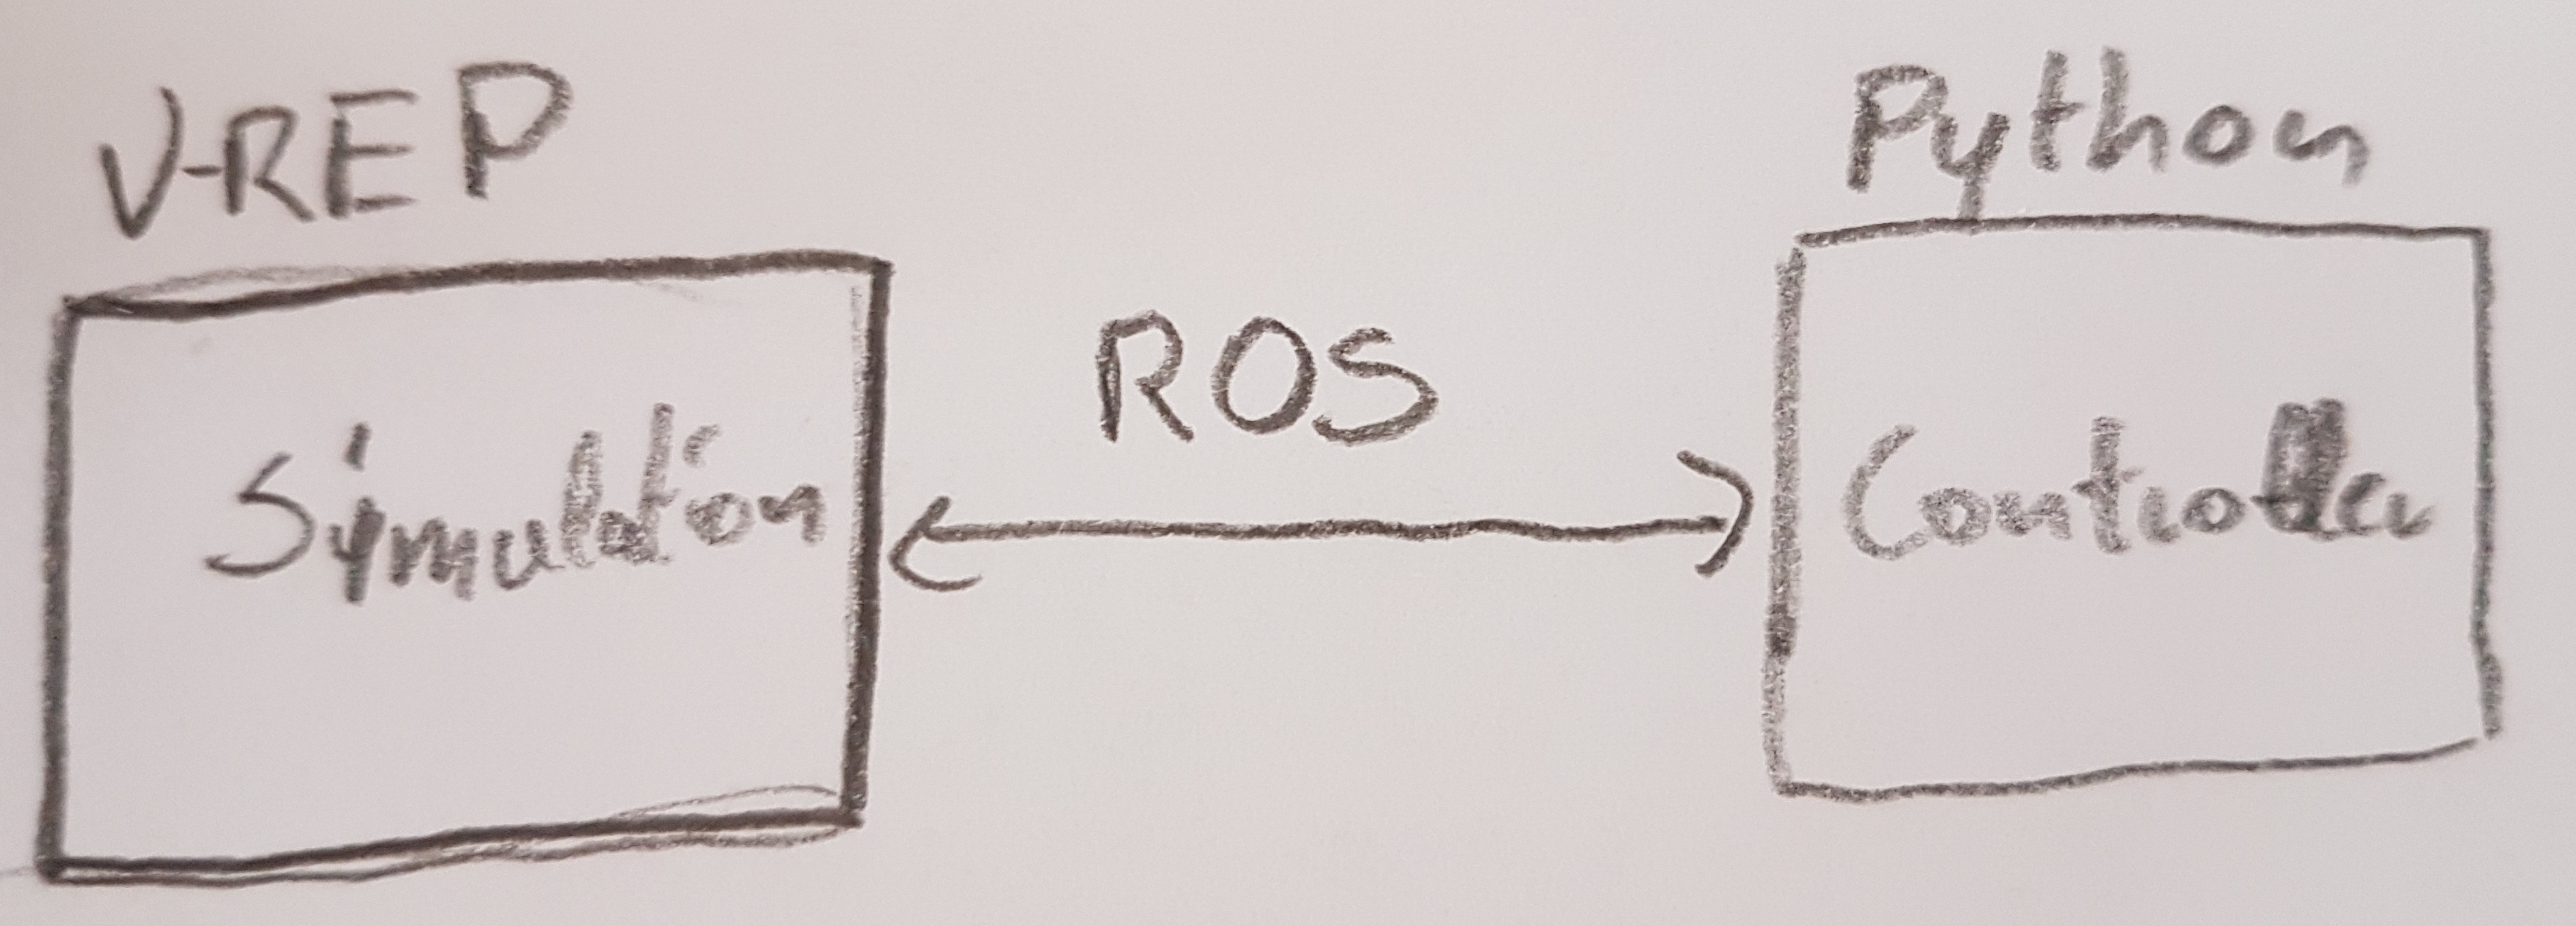
\includegraphics[width=\linewidth]{images/setup.jpg}
	\caption{The two main components and the communication channel}
	\label{fig:setup}
\end{figure}


This section gives a high overview of the experiment. In figure \ref{fig:setup} you can see that there are two main components. First we have the simulation made with V-Rep witch contains the snake like robot and the environment. The environment is made out of a target ball the snake will learn to follow and obstacles in the form of walls. The snake moves according to the movement model from section \ref{section:model}. The second important component is the python controller that will learn to manoeuvre the snake through the environment successfully. The structure of the controller is described in detail in the following section. It contains SNN that will solve a target following and an obstacle avoidance task. The SNN are implemented using the NEST simulator. Both components communicate with each other using ROS. They are both ROS nodes and can exchange messages over the ROS Topic messaging protocol.


\section{Controller}

\begin{figure}
	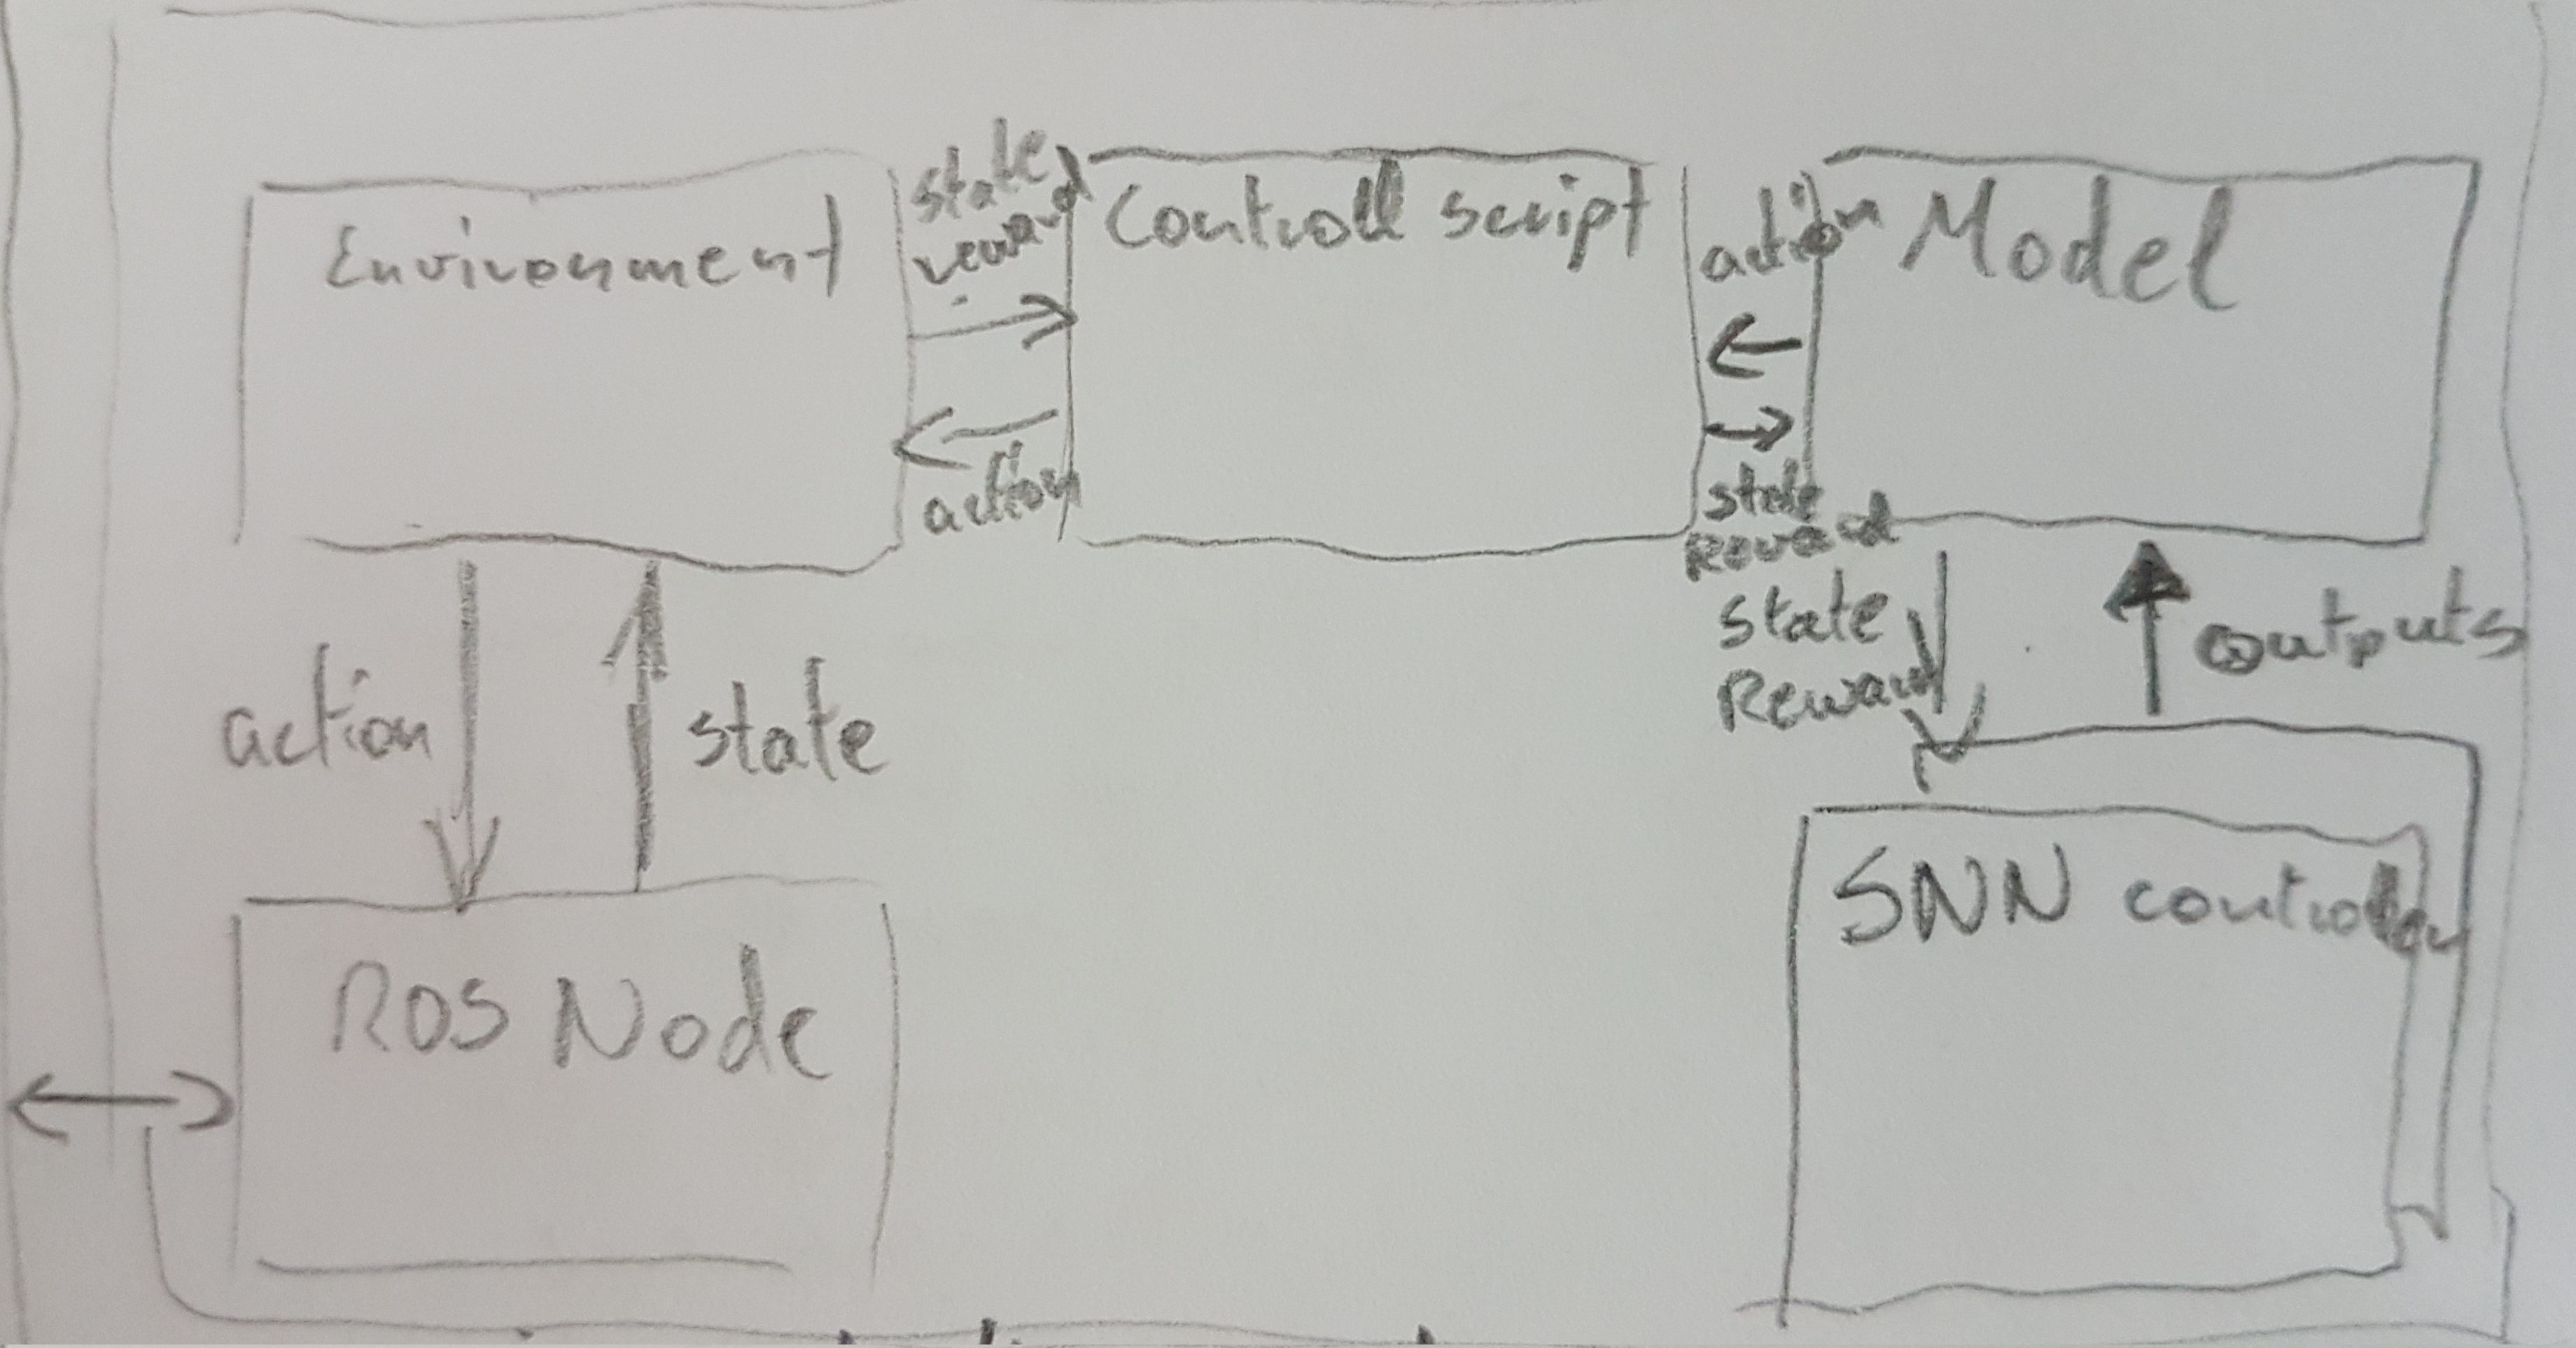
\includegraphics[width=\linewidth]{images/controller.jpg}
	\caption{Architecture of the python controller}
	\label{fig:controller}
\end{figure}

The controller is written in python and distributed over 5 components as can be seen in figure \ref{fig:controller}. Each is implemented in one file. The responsibilities are distributed as follows:

\begin{itemize}
	\item \textbf{Simulation}: The simulation class implements a ROS node and represents the simulation for the controller. All communication with V-Rep goes through this class. Messages are processed and then send to the simulation. Received information gets preprocessed before they are used. It contains the state of the environment as the robot is able to perceive it at a certain moment.
	\item \textbf{Environment}: This class uses the information form the simulation to create a state object. The reward for each output neuron in the SNN's are also calculated here. This class manages changes in the environment like resets.
	\item \textbf{Controll scripts}: They are controlling the experiment flow like if and witch network gets trained. It will also collect data from the environment and the model and save it for later analysis. Examples for these scripts are the training script that will train one model or the controll script that will execute one model for evaluation.
	\item \textbf{Model}: Here the state is feed to the SNN to recive outputs witch then will be interpreted to cosntruct an action that the snake in the simulation will perform.
	\item \textbf{SNN}: The implementation of the SNN network using Nest.
\end{itemize}


\section{Target Following Controller}

The goal of the target following controller is it to successfully follow a target trough the environment. In our simulation the target is represented by a warm ball that can be seen by the infrared camera on the head of the snake.
		
		\chapter{Evaluation}
\label{sec:results}

		
		\chapter{Conclusions and Future Work}
\label{section:conclusions}

		
		% ---------------------------------------------------------------------------
		%
		% Appendix
		%
		% ---------------------------------------------------------------------------
		
		\part*{Appendix}
		\addcontentsline{toc}{part}{Appendix}
		
		\appendix %---------------------------------------
		
		\chapter{Example RDMA application}

%\section{Detailed Validation Results}

\label{chapter:appendixA}


		
	


  \clearemptydoublepage

	\bibliography{bibliography/literature}
	

\end{document}

